\documentclass[12pt]{zettel}

\usepackage{pdfpages}
\usepackage{booktabs}

\usepackage{geometry}
\geometry{tmargin=2cm,bmargin=2cm,lmargin=3cm,rmargin=3cm}

\renewcommand{\gregor}{\put(13.2,-3.0){
\includegraphics[scale=0.18]{cover}}}

\usepackage{framed}
\definecolor{shadecolor}{rgb}{.97,.97,.97}

\begin{document}

\pagestyle{plain}

\renewcommand{\betreff}{}

\makeletterhead{}

\vspace{-2em}

\begin{center}
  \Large\textbf{\textsf{Bewerbung um den Witty-Jugendförderpreis 2014: \\
  Matheschülerzirkel Augsburg}}
\end{center}

XXX: Heißen die so?

Aus der Anforderungsbeschreibung: "`Das Projekt soll
Kindern/Jugendlichen Selbstwertgefühl vermitteln, sie fördern und nachhaltig
Hilfe zur Selbsthilfe bieten."'

\begin{itemize}
\item Information über Verein und Aktivitäten inkl. evtl. Presseberichte
\item Wie setzen sich die rd. 50 TeilnehmerInnen am Mathematikcamp zusammen? Kann
man sich einfach bewerben - läuft es über Lehrer bzw. Schulen?
\item Wie sieht es mit der "`Nachhaltigkeit"' aus? d.h. wie geht es weiter, wenn
einzelne Schüler richtig +Feuer fangen und Begabung zeigen?
\item Wie lauten Ihre Ziele bei diesen Aktivitäten und Projekten? Gibt es zu
wenig Mathematikstudenten und setzen Sie deshalb bereits so früh an?
\item Das Preisgeld beträgt 10.000 Euro. Für das Camp benötigen Sie 7000,--. Wie
würden Sie das restliche Preisgeld sinnvoll verwenden?
\end{itemize}

Der Matheschülerzirkel wurde im September~2013 zur Förderung des
Interesses und der Begeisterung für Mathematik unter Schülerinnen und Schülern
an weiterführenden Schulen gegründet. Während des Schuljahrs~2013/2014 betreuen
etwa 15~Mitarbeiterinnen und Mitarbeiter ehrenamtlich die knapp
250~teilnehmenden Schülerinnen und Schüler in zweiwöchentlich an der
Universität stattfindenden Seminaren. Für weiter entfernt wohnende Schülerinnen
und Schüler unterhalten wir monatliche Korrespondenz per Post.

Als nächstes großes Projekt führen wir ein fünftägiges Mathecamp in den
Sommerferien~2014 durch. Die Angebote des Matheschülerzirkels sind in Augsburg
und Schwaben einzigartig und sollen langfristig weitergeführt und ausgebaut
werden.


\section{Bewerber}

Wir sind Mitarbeiterinnen und Mitarbeiter des Instituts für Mathematik der
Universität Augsburg. Wir verfügen über ein abgeschlossenes Mathematik-Studium
und promovieren nun in Mathematik. Durch unser junges Alter können wir auf
einer XXX Ebene gut mit Schülerinnen und Schülern kommunizieren.

XXX Wir haben Erfahrung in Jugendarbeit.


\section{Vision}

Das Hauptziel des Mathezirkel Augsburg ist es, Schülerinnen und Schülern
langfristig eine Möglichkeit zu bieten, ihrem Interesse an der
Mathematik nachzugehen. Wir möchten Kindern, die frühzeitig Spaß an der
Mathematik gefunden haben, dazu animieren und darin unterstützen, ihre
BegabungenXXXzustark? weiterzuentwickeln.
Es geht uns darum, diesen Schülerinnen und
Schülern zu zeigen, wie spannend Mathematik sein kann und wie diese außerhalb der Schule aussieht. 

Wenn Schulkinder an Musik oder Sport interessiert sind, haben sie immer die
Möglichkeit, darin gefördert zu werden oder einem Verein beizutreten. Für
Mathematik gibt es dagegen kaum Angebote außerhalb des Unterrichts. Aus diesem
Grund geht das Interesse an Mathematik, dass viele Kinder im Grundschulalter
noch haben, in den folgenden Jahren leider oft verloren. Hier wirken wir
dagegen. Deshalb ist es uns sehr wichtig, früh genug an die Jugendlichen
heranzutreten und ihr Mathematikinteresse über viele Schuljahre
Schuljahre hinweg zu erhalten.

In diesem Sinne verstehen wir uns als Förderer der MINT-Bildung von
Jugendlichen. XXX etwas verloren

Ein wichtiger Punkt zur Unterstützung des Interesses an der
Mathematik, welcher auch für sich selbst bereits erstrebenswert ist, ist es,
Schülerinnen und Schülern mit Spaß an der Mathematik zusammenzubringen.
An einer einzigen Schule finden sich vielleicht
nur ein oder zwei Jugendliche, in Augsburg und Schwaben sind es jedoch
deutlich mehr. Durch regelmäßige Treffen und Feriencamps lernen die
Kinder Gleichgesinnte kennen, was ihnen enorm viel Freude bereiten kann.

Unser primäres Ziel ist nicht, Schülerinnen und Schüler zu einem
Mathematik-Studium zu bewegen. Viel wichtiger ist uns, Interesse und
Begeisterung an Mathematik zu wecken und zu erhalten. Während unsere Kompetenz
in der Mathematik liegt und wir daher nur dafür Förderprojekte anbieten können,
hat unsere Arbeit auch für die anderen MINT-Bereiche eine Bedeutung.
Schließlich wird Mathematik in allen Naturwissenschaften, der Informatik und
der Technik eingesetzt. Jugendlichen, die Spaß an Mathematik haben, steht ein
breites Spektrum interessanter Studien- und Berufsmöglichkeiten zur Verfügung.
XXX


\section{Projektbeschreibung}

Der Matheschülerzirkel Augsburg besteht aus mehreren einander ergänzenden Veranstaltungen, die im
Folgenden einzeln beschrieben werden. Interessierte Schülerinnen und Schüler
können diese unabhängig voneinander besuchen. Bis auf das Mathecamp sind alle
Veranstaltungen für die Teilnehmenden kostenlos.

In Bayrisch-Schwaben gibt es vereinzelte, deutlich kleinere lokale
Projekte, die ähnlich wie wir auf Mathematikförderung bei Schülerinnen und
Schülern ausgerichtet sind. Diese sind aber entweder nur an einzelnen Schulen
angesiedelt und stehen daher nur wenigen Jugendlichen zur Verfügung oder zielen
auf Mathematiknachhilfe ab. Der Matheschülerzirkel Augsburg ist das erste
Projekt auf diesem Gebiet, das unabhängig von schulischen Leistungen die
Begeisterung für Mathematik fördern und erhalten möchte und sich auf die
BegabungsförderungXXXzustark konzentriert.

An anderen Orten wie Leipzig und Stuttgart werden ähnliche Projekte seit
vielen Jahren erfolgreich durchgeführt. Der überwältigende Ansturm in
diesem Schuljahr zeigte, dass auch hier in Augsburg und Umgebung Nachfrage
besteht.

XXX Hier zu Beginn betonen, dass es nicht um Nachhilfe geht.


\subsection{Präsenzzirkel}

Die insgesamt zehn Präsenzzirkel finden in nach Klassenstufe eingeteilten
Kleingruppen von fünf bis zehn Schülerinnen und Schülern statt.
Die jeweilige Gruppe trifft sich alle zwei Wochen mit ihrer Zirkelleiterin oder ihrem
Zirkelleiter auf dem Campus der Universität Augsburg und diskutiert und
bearbeitet in gut 90~Minuten Themen der Mathematik, die außerhalb des
Schulstoffs liegen. Durch die kleine Gruppengröße können wir individuell auf
Vorkenntnisse und Themenwünsche eingehen.

Der Ablauf eines Präsenzzirkels hängt stark von der Klassenstufe ab. Bei den
niedrigen Klassenstufen werden Themen eher durch Bearbeiten von passenden
Aufgaben in Eigeninitiative erkundet, während Schülerinnen und Schüler höherer
Klassenstufen auch durch geleitete Diskussionen in der Gruppe
Themen erarbeiten können. In vielen Zirkeln finden spezielle Materialien,
wie zum Beispiel Zauberwürfel, selbstgeschriebene Computerprogramme oder
BastelutensilienXXX Verwendung.

Die Themen sind sehr vielfältig, sie reichen unter anderem von
Knobelaufgaben, geheimen Botschaften, Fibonacci-Zahlen und Nim-Spielen (ab Klasse 5),
über Zahlentheorie, Geometrie und Zauberwürfeln (ab Klasse 7) bis hin zu
Fraktalen und Chaos, vierdimensionaler Geometrie und nichtklassischer Logik
(ab Klasse 9). Wir bereiten auch auf mathematische Wettbewerbe vor. 

Die Präsenzzirkel bieten den Teilnehmerinnen und Teilnehmern die Möglichkeit,
gemeinsam mit weiteren mathematisch interessierten Jugendlichen außerhalb der
Schule Mathematik zu betreiben. Die Zirkel finden außerhalb der Schulzeiten
statt und ist für die Schülerinnen und Schüler kostenlos. Der Einstieg ist
jederzeit möglich.


\subsection{Korrespondenzzirkel}

Viele unserer Schülerinnen und Schüler können aus verschiedenen Gründen
nicht zu unseren Präsenzzirkeln kommen, beispielsweise, weil sie zu weit
entfernt von Augsburg wohnen oder andere Termine haben.
Daher bieten wir auch schriftliche Korrespondenzzirkel per Post
an.

Genau wie die Präsenzzirkel sind diese nach Klassenstufen eingeteilt. Ein
Korrespondenzbrief enthält ein kurzes, von der Zirkelleiterin oder dem
Zirkelleiter geschriebenes Skript zu einem mathematischen Thema sowie passende
Übungsaufgaben. Die Jugendlichen haben pro Brief etwa vier Wochen Zeit, um sich
mit dem Stoff auseinanderzusetzen, die Aufgaben zu lösen und ihre Ergebnisse
zurückzuschicken. Die Zirkelleiterinnen und Zirkelleiter senden dann
ausführliche Korrekturen und Tipps zurück.

Thematisch ähneln sich die beiden Zirkelarten. Außerdem ist genau wie bei den
Präsenzzirkeln der Einstieg jederzeit möglich.


\subsection{Mathecamp}

Als drittes großes Projekt führen wir vom 16. bis 20. August erstmals ein
mathematisches Sommercamp durch. Dabei ermöglichen wir etwa 60~Teilnehmerinnen
und Teilnehmern, sich intensiv mit einer Auswahl mathematischer Themen zu
beschäftigen und Gleichgesinnte kennenzulernen.

Dafür haben wir das Bruder-Klaus-Heim der Diözese Augsburg in Violau
gebucht. An jedem Tag beschäftigen sich die Schülerinnen und Schüler in zwei
Arbeitseinheiten mit Themen, die in den Präsenz- und Korrespondenzzirkeln noch
nicht behandelt wurden. Selbstverständlich sind auch diese Kurse nach dem Alter
und den Vorkenntnissen der Teilnehmenden abgestuft. Ferner
werden eine auswärtige Mathematikerin und ein Mathematiker zwei Vorträge halten.

Für die restliche Zeit bietet unsere Unterkunft ein reichhaltiges
Freizeitangebot. Das ist eine gute Gelegenheit für die Jugendlichen,
sich mit ähnlich Interessierten auszutauschen. XXX

Das Camp steht allen mathematisch interessierten Schülerinnen und Schülern der
Klassenstufen~5 bis~12 offen, auch solchen, die unsere anderen Angebote bisher
nicht wahrgenommen haben. Bei der Vorankündigung stieß das Camp auf große
Begeisterung. Die offizielle Anmeldephase begann am 10. Juni 2014.

Als einziges unserer Projekte können wir das Mathecamp nicht kostenlos
anbieten. Wir benötigenXXX eine Eigenbeteiligung von 70~\texteuro{} pro
Teilnehmenden. Die uns tatsächlich entstehenden Kosten liegen bei etwa
200~\texteuro{} pro Teilnehmenden.

XXX zu kurz?


\subsection{Matheolympiade}

Im Februar 2015 werden wir auf dem Campus der Universität die Landesrunde der deutschen
Mathematikolympiade für Klassenstufen~5 und~6 von Schulen im Großraum
Augsburg durchführen. Die Mathematikolympiade ist ein internationaler mathematischer
Klausurwettbewerb, deren mehrstufige Auswahlklausuren für die Bundesrunde
bislang dezentral an den einzelnen Schulen durchgeführt wurden. Seit einigen
Jahren gibt es zentrale Landesrunden für die Klassenstufen~7 und höher, die von
MOBy~e.\,V. organisiert werden.

Da es aber insbesondere für Schülerinnen und Schüler aus den Klassenstufen~5
und~6 etwas ganz Besonderes ist, für ihre Erfolge in der zweiten Stufe
eingeladen zu werden und die Klausur der Landesrunde gemeinsam mit anderen
Teilnehmerinnen und Teilnehmern zu schreiben, möchten wir diese Veranstaltung
ins Leben rufen.

Dazu laden wir im Februar 2015 ungefähr~50 der in der zweiten Stufe
erfolgreichsten Fünft- und Sechstklässlerinnen und -klässler des Großraums
Augsburg zu uns ein. Diese schreiben dann gemeinsam ihre Olympiadeklausur und
können sich am Nachmittag während der Korrektur unter Betreuung kennenlernen
und austauschen. Abschließend gibt es eine offizielle Siegerehrung.

Eine zentrale Landesrunde ist eine gute Möglichkeit, die sonst von
Hausaufgabenwettbewerben geprägte Mathematikwettbewerbslandschaft durch
Klausurwettbewerbe zu erweitern und dadurch mathematikbegeisterte Schülerinnen
und Schüler zusammenzuführen. Solche für die Schülerinnen und Schüler
sehr besonderen Erfahrungen steigern auch ihr Selbstwertgefühl. Sie zeigen
den Jugendlichen, dass ihre Begeisterung für Mathematik geschätzt wird. XXX

Wir hoffen, dass sich dadurch auch die Teilnahmequote
in den höheren Klassenstufen langfristig erhöht.


\subsection{Weitere Aktivitäten}

Neben den bereits genannten Zirkeln, dem Mathecamp und der
Matheolympiade organisieren wir noch weitere kleinere
Aktivitäten.

Die wichtigsten zwei Veranstaltungen dieser Art sind die Auftakt- sowie die
Abschlussveranstaltung. Am 09.11.2013 fand unsere erste
Auftaktveranstaltung mit einem anschaulichen und für alle Klassenstufen
geeigneten Vortrag von
Prof.~Dr.~Jost-Hinrich Eschenburg zum Thema \emph{Was sind eigentlich die
Zahlen?} statt.
Die über 150 Teilnehmerinnen und Teilnehmer und deren Eltern waren durchweg
begeistert. Nach einer Stärkung für die Besucher führten wir
die Anmeldung und Terminplanung der Zirkel durch.

Am Ende des Schuljahres wird es eine Abschlussveranstaltung mit einem
weiteren mathematischen Vortrag geben, bei der wir
das vergangene Jahr in den Zirkeln Revue passieren lassen und als Anerkennung
mathematische Kleingeschenke verteilen. Diese beiden Veranstaltungen sollen
auch in den kommenden Jahren dem Schuljahr einen Rahmen geben.

Des Weiteren besuchen wir mit unseren Präsenzzirkelteilnehmern die
Vortragsreihe Fanszination Mathematik und Physik, in welcher viermal im
Jahr Mathematikerinnen und Mathematiker sowie Physikerinnen und Physiker in Augsburg ihre Forschung der
Öffentlichkeit anschaulich darlegen. Weiterhin unterstützen wir
Mathematik betreffende Aktionen wie den Tag der Mathematik an
der Universität Augsburg oder den Girl's Day.

Im kommenden Schuljahr möchten wir Wochenendtreffen für die Teilnehmerinnen und
Teilnehmer der Korrespondenzzirkel anbieten, um auch diesen Jugendlichen die
Möglichkeit zu bieten, sich mit Gleichgesinnten auszutauschen. Diese Treffen
sollen etwa zweimal pro Jahr stattfinden.

Außerdem möchten wir an mehreren Wochenenden einzelne Vorträge in einem
größeren Rahmen anbieten, vorrangig für Schülerinnen und Schüler aus Augsburg.
Die Vorträge sollen von auswärtigen Mathematikerinnen und Mathematikern aus
Wirtschaft und Wissenschaft gehalten werden.


\section{Zielgruppe}

Unser Projekt richtet sich an mathematisch interessierte Schülerinnen
und Schüler der Klassenstufen 5 bis 12. Die einzige Voraussetzung zur
Teilnahme ist Spaß und Interesse an der Mathematik. Es gibt insbesondere
keine Noten, Schulzugehörigkeiten oder Wettbewerbsergebnisse als
Beschränkung, denn Spaß an der Mathematik
ist unabhängig von Schulergebnissen oder der Teilnahme an
Wettbewerben.

Im letzten Jahr sahen wir, dass die meisten unserer Kinder eine
sehr hohe Motivation für Mathematik mitbrachten und neugierig auf die
Mathematik außerhalb der Schule waren. Alle Jugendliche, die Interesse an
Rätseln, Logik und abstraktem Denken mitbringen, bilden unsere
Zielgruppe.

Es zeigte sich, dass der Großteil unser Schülerinnen und
Schüler Gymnasien besucht, aber auch einige Realschülerinnen teilnehmen.
Auch Fachoberschülerinnen und "~schülern steht unser Angebot offen, im nächsten
Jahr möchten wir dort verstärkt werben.

Etwa zwei Drittel unserer Teilnehmenden
stammen aus den Klassenstufen~5 bis~8. 
Dies deckt sich mit der
Erfahrung von anderen Orten, dass anfangs ein größeres Interesse für
Mathematik besteht und dieses oft im Laufe der Pubertät
deutlich nachlässt -- ein Problem, dem wir gezielt begegnen.

Ein weiteres bekanntes Problem im MINT-Bereich
und der Mathematik im Speziellen ist der niedrige Frauenanteil in
Studium und Beruf. Deshalb freut es uns sehr, dass 40~Prozent unserer
Teilnehmer weiblich sind. In den Klassenstufen~5 und~6 ist die Quote sogar
ausgeglichen. Wir hoffen, die dort teilnehmenden Mädchen weiterhin für die
Mathematik motivieren zu können.

In den Korrespondenzzirkeln betreuen wir Schülerinnen und Schüler aus ganz
Schwaben, sowie vereinzelt darüber hinaus. Dagegen kommen die Teilnehmerinnen
und Teilnehmer der Präsenzzirkel alle aus dem Großraum Augsburg. Viele davon
nehmen sogar an beiden Zirkeln teil.

Nachhilfeangebote für Schülerinnen und Schüler, die sich mit der Mathematik
schwer tun, sind ebenfalls wichtig, gehören aber nicht zu unserem
Aufgabengebiet. Gerade im Großraum Augsburg gibt es schon mehrere Firmen und
Institutionen, die diesen Bereich abdecken. Außerdem ist für solche
Schülerinnen und Schüler oftmals private Nachhilfe durch Bekannte eine gute
Option. XXX


\section{Budget}

Wir selbst arbeiten ehrenamtlich. Finanzielle Unterstützung benötigen wir aber
für die von uns durchgeführten Veranstaltungen. Die Professoren und
Professorinnen des Instituts für Mathematik stehen voll hinter unserem Projekt
und ermöglichen uns, unentgeltlich die Räumlichkeiten der Universität zu nutzen
und organisatorische Ausgaben wie Briefporto über das Institut abzurechnen.
So entstehen uns für die Präsenz- und Korrespondenzzirkel keine Kosten, und
daher können wir diese auch den Schülerinnen und Schülern unentgeltlich
anbieten.

Aus rechtlichen Gründen kann das Institut den Matheschülerzirkel aber leider nicht
direkt finanziell unterstützen, denn wir können weder unter dem Posten
\emph{Lehre} verbucht werden, da unsere Schüler nicht an der Universität
immatrikuliert sind, noch unter den Posten \emph{Werbung}, da die Zirkel und
das Mathecamp keine Werbeveranstaltungen sein sollen -- obwohl sie natürlich indirekt
durchaus zu einem Aushängeschild der Universität werden können.

Um unser Projekt langfristig durchführen zu können, sind wir daher auf externe
Fördermittel angewiesen.

Weiter unten sind in tabellarischer Form unsere geplanten Ausgaben für ein
typisches Schuljahr aufgeführt. In diesem Schuljahr konnten wir
neben den Präsenz- und Korrespondenzzirkeln nur die Auftaktveranstaltung
realisieren. Für das in diesem August
stattfindende Mathecamp haben wir über \emph{Bündnis für Augsburg} und ein
Drittmittelprojekt eine einmalige Finanzierungsmöglichkeit gefunden, die
allerdings keine langfristige Option darstellt und nur ein Minimalprogramm mit 40~Teilnehmerinnen und
Teilnehmer abdeckt. Ohne zusätzliche Finanzierung müssten wir weiteren
Interessenten leider absagen. Außerdem könnten wir einkommensschwache Familien
kaum unterstützen.

Sollten wir den Förderpreis erhalten, wäre die Finanzierung des Mathecamps in
voller Höhe gesichert. Außerdem könnten wir sicher unsere für das nächste Schuljahr
geplanten Veranstaltungen durchführen; nur für den vollen Umfang des
Camps bräuchten wir dann noch zusätzliche Unterstützung. Wir könnten außerdem
eine einmalige Investition in so genannte \emph{dynamische Labyrinthe} tätigen --
das sind etwas teurere Materialien, mit denen man
Computerprogrammierung anschaulich und auch für Schülerinnen und Schüler niedriger Klassenstufen
verständlich erklären kann.


\begin{center}\small
\renewcommand{\arraystretch}{1.3}
\begin{tabular}{@{}p{5.7cm}@{\qquad}r@{\qquad}p{6cm}@{}}
  \toprule
  \multicolumn{3}{@{}l@{}}{\textbf{Jahresbudget pro Schuljahr}} \\
  \toprule
  \textbf{Auftaktveranstaltung mit 150 Schülern und deren Eltern} & circa 500 \texteuro & im September \\
  Verpflegung & 400 \texteuro \\
  Flyer und Plakate & 100 \texteuro \\\\
  \textbf{Materialien für Präsenz- und Korrespondenzzirkel} & circa 1.500 \texteuro &
  Bücher zur Kursvorbereitung,
  Bastel- und Anschauungsmaterialien \\\\
  \textbf{Treffen der Korrespondenzzirkelteilnehmer} &
  circa. $2 \times 300$ \texteuro &
  zwei Mal im Jahr, geplant ab Schuljahr 2014/2015 \\\\
  \textbf{Vortragssamstage} &
  circa. $2 \times 300$ \texteuro &
  zwei Mal im Jahr, geplant ab Schuljahr 2014/2015 \\\\
  \textbf{Mathematikolympiade mit 50 Teilnehmern} & circa 1.500 \texteuro &
  im Februar \\\\
  \textbf{Abschlussveranstaltung mit 100 Schülern und deren Eltern} & circa 700 \texteuro &
  im Juli \\
  Verpflegung & 300 \texteuro \\
  Preise und Urkunden & 400 \texteuro \\\\
  \textbf{Mathecamp \phantom{aaaaaaaaaaaaaa} mit 60 Teilnehmern} & circa 7.100 \texteuro \\
  Unterkunft mit Verpflegung & 8.908 \texteuro & 30 \texteuro{} pro Nacht und
  Person zzgl. 11 \texteuro{} Mittagessen am letzten Tag
  (60 Teilnehmer und 8 Betreuer) \\
  An- und Abreise & 300 \texteuro & Busunternehmen \\
  Versicherung & 170 \texteuro & 2,50 \texteuro{} pro Person \\
  Sonstiges & 1.500 \texteuro & Workshop-Materialien,
  Zwischenmahlzeiten, Freizeitaktivitäten, Benzinkosten eines Autos vor Ort,
  diverse kleinere Posten \\
  Eigenbeteiligung & $-$3.800 \texteuro & 70 \texteuro{} pro Kind
  (abzüglich 400 \texteuro{} an Zuschüssen für einkommensschwache Familien) \\
  \bottomrule
  \textbf{Summe} & circa 12.500 \texteuro \\
  \bottomrule
\end{tabular}
\end{center}


\section{Öffentlichkeitsarbeit}

Um auf die Initiierung unseres Projekts zu Beginn des Schuljahrs~2013/2014
aufmerksam zu machen, schickten wir allen Gymnasien Schwabens und einigen
weiteren Schulen im Umkreis von Augsburg Informationspakete mit Lehrerbriefen,
Flyern und Plakaten. Um sicherzugehen, dass unser Angebot in der
Vielzahl der Korrespondenz bei den Schulen nicht unterging, befragten wir außerdem
die Studenten der Universität nach Lehrern, die zu ihrer Schulzeit
besonders großes Engagement zeigten, und schrieben diese separat an.
Häufig zeigten sich diese sehr angetan von unserem Projekt.

Ferner unterstützte uns bei der Öffentlichkeitsarbeit das Kultusministerium,
unter anderem dadurch, indem dass es zusätzlich zu unseren Briefen einen Aufruf zur
Beteiligung auch noch einmal direkt an die Schulen weiterleitete.

Schließlich gaben wir eine Pressemitteilung heraus, die von der
Augsburger Allgemeinen aufgegriffen und zu einem prominenten Artikel aufbereitet
wurde (siehe Anlage). Als das Projekt angelaufen war, kam das Augsburger
Regionalfernsehen a.tv auf uns zu und drehte eine kurze Reportage
(\href{http://www.augsburg.tv/aktuell/schuelerzirkel-mathematik-30_12_2013.html}{\textsf{http:/\!/www.augsburg.tv/aktuell/schuelerzirkel-mathematik-30\_{}12\_{}2013.html}}).

Auf diese Weise konnten wir insgesamt etwa~250 Schülerinnen und Schüler für
unser Projekt begeistern, davon etwa~120 aus dem Großraum Augsburg. Um Werbung für
das Mathecamp zu machen, nutzen wir vor allem den bereits etablierten Kontakt
und informieren unsere Schülerinnen und Schüler in den Seminaren persönlich und
zusätzlich per Brief. Ferner verfassen wir wieder eine Pressemitteilung und
benachrichtigen die Augsburger Allgemeine.

Selbstverständlich sind wir auch im Internet auf den Seiten der Universität
vertreten
(\href{http://www.math.uni-augsburg.de/schueler/mathezirkel/}{\textsl{http:/\!/www.math.uni-augsburg.de/schueler/mathezirkel/}})
und schülerfreundlich über Facebook zu erreichen. Über den
Mathematisch-Physikalischen Verein~e.\,V. erreichen wir Alumni und Freunde der
Universität.


\section{Zeitrahmen}

Der Matheschülerzirkel Augsburg begann im Schuljahr 2013/2014 mit der
Eröff\-nungs\-ver\-an\-stal\-tung am 09.11.2013. Die Organisation für das Projekt
startete bereits Anfang August 2013. Diese Zirkel und
das Sommercamp werden ein fester Bestandteil des Instituts für Mathematik und
der Arbeit des Mathematisch-Physikalischen Vereins e.\,V.

Die Korrespondenz- und Präsenzzirkel laufen
das gesamte Schuljahr über. Sie werden von einer
Eröffnungsveranstaltung am Anfang und von einer
Abschlussveranstaltung am Ende des Schuljahres umrahmt. Das Mathecamp soll
einmal jährlich in den Sommerferien stattfinden. Die dritte Stufe der
Matheolympiade für Klassenstufen~5 und~6 findet einmal pro Jahr
im Februar statt und wir planen, diese in
Absprache mit \emph{Mathematik-Olympiade in Bayern e.\,V.} in Augsburg
durchzuführen.

Das Mathecamp wird dieses Jahr fünf Tage dauern. Wir hoffen, dass die
Teilnehmenden so begeistert sein werden,
dass wir in den nächsten Jahren das
Mathecamp zeitlich ausdehnen können. Erfahrungen aus
anderen Regionen zeigen, dass diese Hoffnung durchaus berechtigt ist.

Neben diesen Hauptprojekten möchten wir unseren Schülerinnen und
Schülern weitere Angebote machen, welche ebenfalls permanent angeboten
werden sollen. Dazu gehören Besuche der Vortragsreihe Faszination
Mathematik und Physik in Augsburg, Teilnahmemöglichkeiten
an Mathematikwettbewerben und Mathematikschulveranstaltungen der Universität Augsburg.

Da unser Projekt langfristig ausgelegt ist, viele der jetzigen Doktoranden und
Mitarbeiter in einigen Jahren aber aus der Universität ausscheiden werden,
bemühen wir uns schon jetzt um Verstärkung.
Dazu integrieren wir das Projekt so gut wie möglich mit
dem Institut und dem Verein, sodass auch permanente Beschäftigte,
insbesondere Professorinnen und Professoren, mithelfen. Daneben sprechen wir
aktiv junge Studierende an, um diese auf die Zirkelarbeit
vorzubereiten und zu motivieren, den Matheschülerzirkel
Augsburg in die Zukunft zu führen.


\section{Ansprechpartner}

Die Hauptorganisatoren sind Ingo Blechschmidt, Kathrin Helmsauer und Sven
Prüfer. Sie erreichen uns telefonisch unter 0821/598-5601, 0821/598-5795 bzw.
0821/598-5805. Eine allgemeine E-Mail-Adresse, die uns alle erreicht, ist
\textsf{mathezirkel@math.uni-augsburg.de}. Unsere persönlichen Adressen sind
\textsf{ingo.blechschmidt@math.uni-augsburg.de},
\textsf{kathrin.helmsauer@math.uni-augsburg.de} bzw.
\textsf{sven.pruefer@math.uni-augsburg.de}. Unsere Post-Anschrift lautet:

\begin{tabbing}
  Matheschülerzirkel Augsburg \\
  Lehrstuhl für Algebra und Zahlentheorie \\
  Universitätsstraße 14 \\
  86159 Augsburg
\end{tabbing}


\section{Erfolgskontrolle}

Unmittelbar und rein qualitativ können wir den Erfolg an den Rückmeldungen der
Kinder und ihrer Eltern messen: Bereitet den Kindern der Präsenzzirkel, der
Korrespondenzzirkel und das Camp Spaß, Freude und Interesse? Gibt es
Verbesserungsvorschläge, Wünsche für das Folgejahr oder anderweitige Kritik?

Quantitativ können wir unseren Erfolg anhand der Teilnehmerzahlen im nächsten
Jahr messen: Wenn den Kindern unsere Veranstaltungen gefallen, werden sie sich
nächstes Jahr wieder anmelden und vielleicht sogar Freunde mitbringen.

Langfristig können wir auch verfolgen, wie viele unsere Teilnehmer später ein
Studium in den Bereichen Mathematik, Informatik, Naturwissenschaft und Technik
beginnen. Auf die Steigerung von solchen Studienzahlen legen wir aber kein
besonderes Augenmerk -- andere Fächer sind ja ebenfalls interessant! Wichtiger
ist uns, die jetzt vorhandende Begabung und das Interesse zu fördern. XXX ganz
ganz schlecht!
Vorschlag Steffie:
Langfristig... Es wäre natürlich schön, wenn einige unserer Schüler durch
unsere Arbeit so für den MINT-Bereich begeistert werden, dass sie dort ein
Studium beginnen. Auf die alleinige Steigerung solcher Studienzahlen kommt es
uns aber wie bereits erwähnt nicht an. Wichtig ist uns, die jetzt vorhandene
Begabung und das Interesse zu fördern, so dass lebenslang eine Begeisterung für
die Mathematik herrscht und sie diese auch an andere weitergeben können.
super schnulzig

Interessant wird auch, zu beobachten, wie sich die Beteiligung an
mathematischen Wettbewerben entwickelt. Wird sich die Zahl der
Teilnehmerinnen und Teilnehmer aus Augsburg und Schwaben am Landeswettbewerb
Mathematik Bayern, am Bundeswettbewerb Mathematik und an der deutschen
Mathematikolympiade durch uns erhöhen? Wir sind bereits erfreut,
dass sich in diesem Jahr vier unserer Schülerinnen und Schüler für die
Bundesrunde der Mathematikolympiade qualifizierten.

In unserem ersten Jahr erhielten wir auch schon sehr positive Rückmeldungen der
Kinder und Eltern. BestätigungXXX der Präsenzzirkel erhielten wir insofern, als
dass sie im Laufe des Jahres immer gut besucht blieben.

XXX Erwähnen: Buchführung und Einarbeiten von Erkenntnissen in Zukunft.
Austausch unter den Zirkelleitern

XXX Nicht nur Fragen formulieren, sondern konkret sagen, dass bereits
Rückmeldungen stattgefunden haben?!

XXX emph

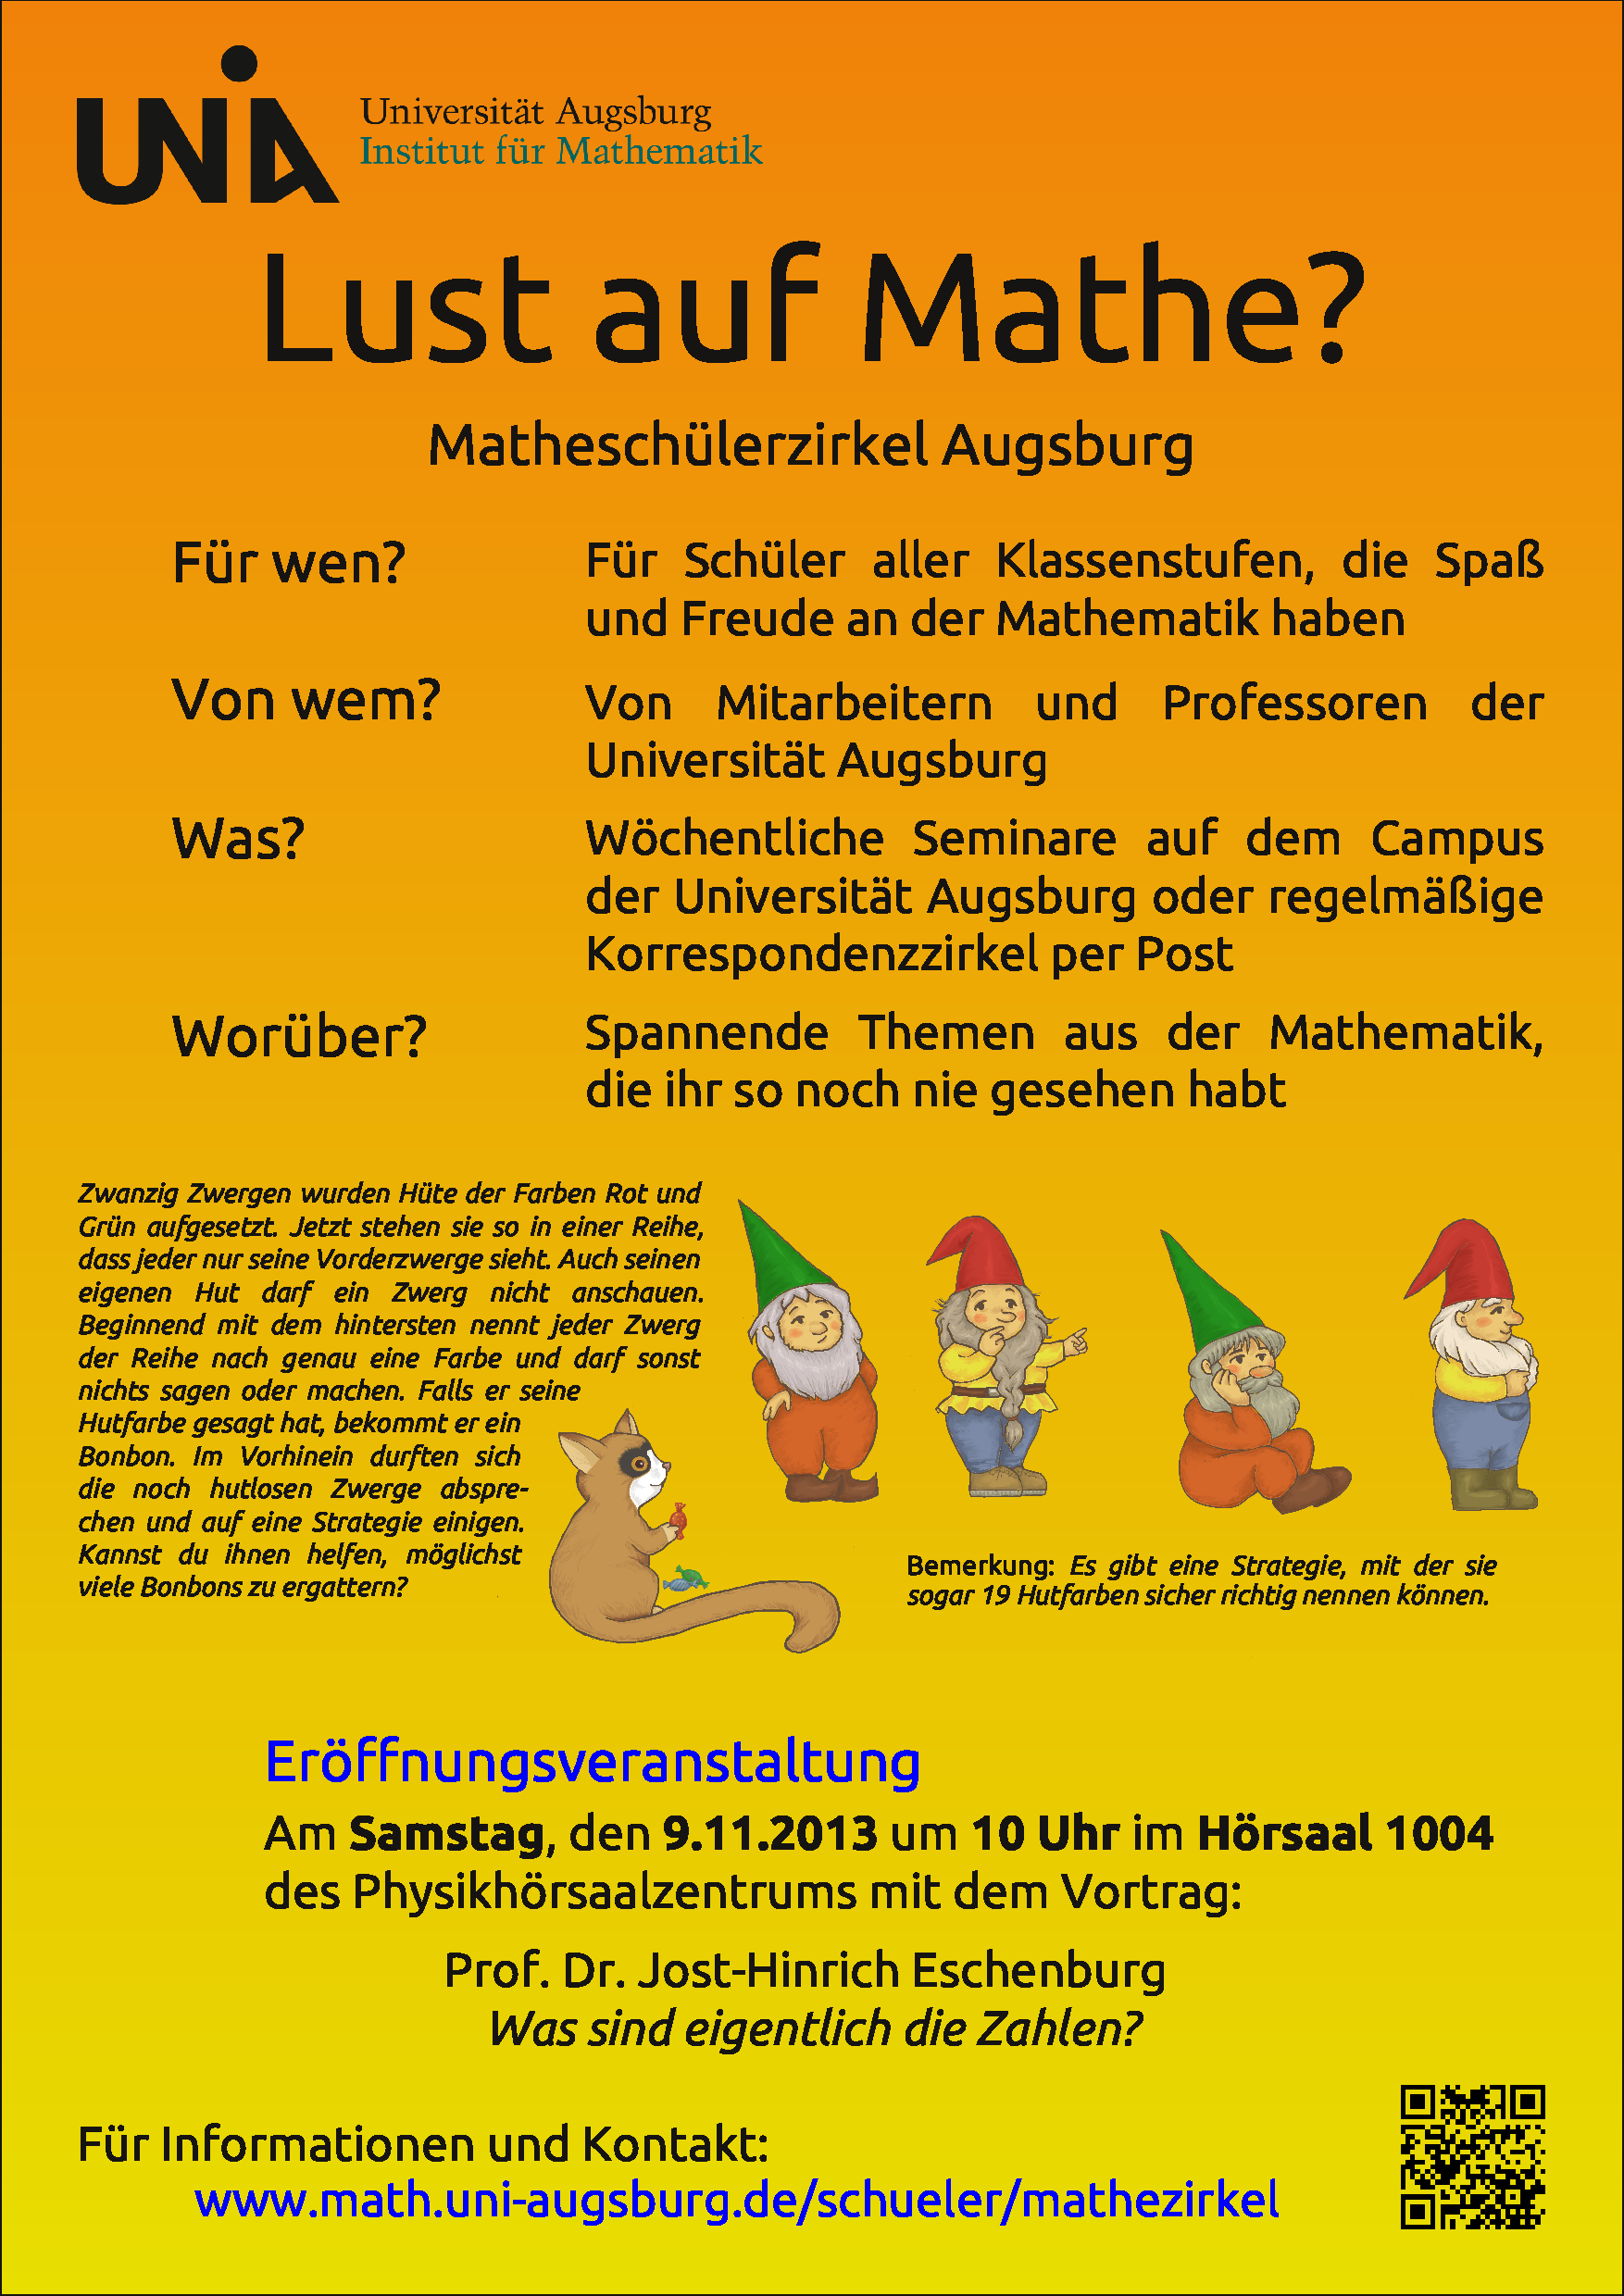
\includepdf{poster_mathezirkel}

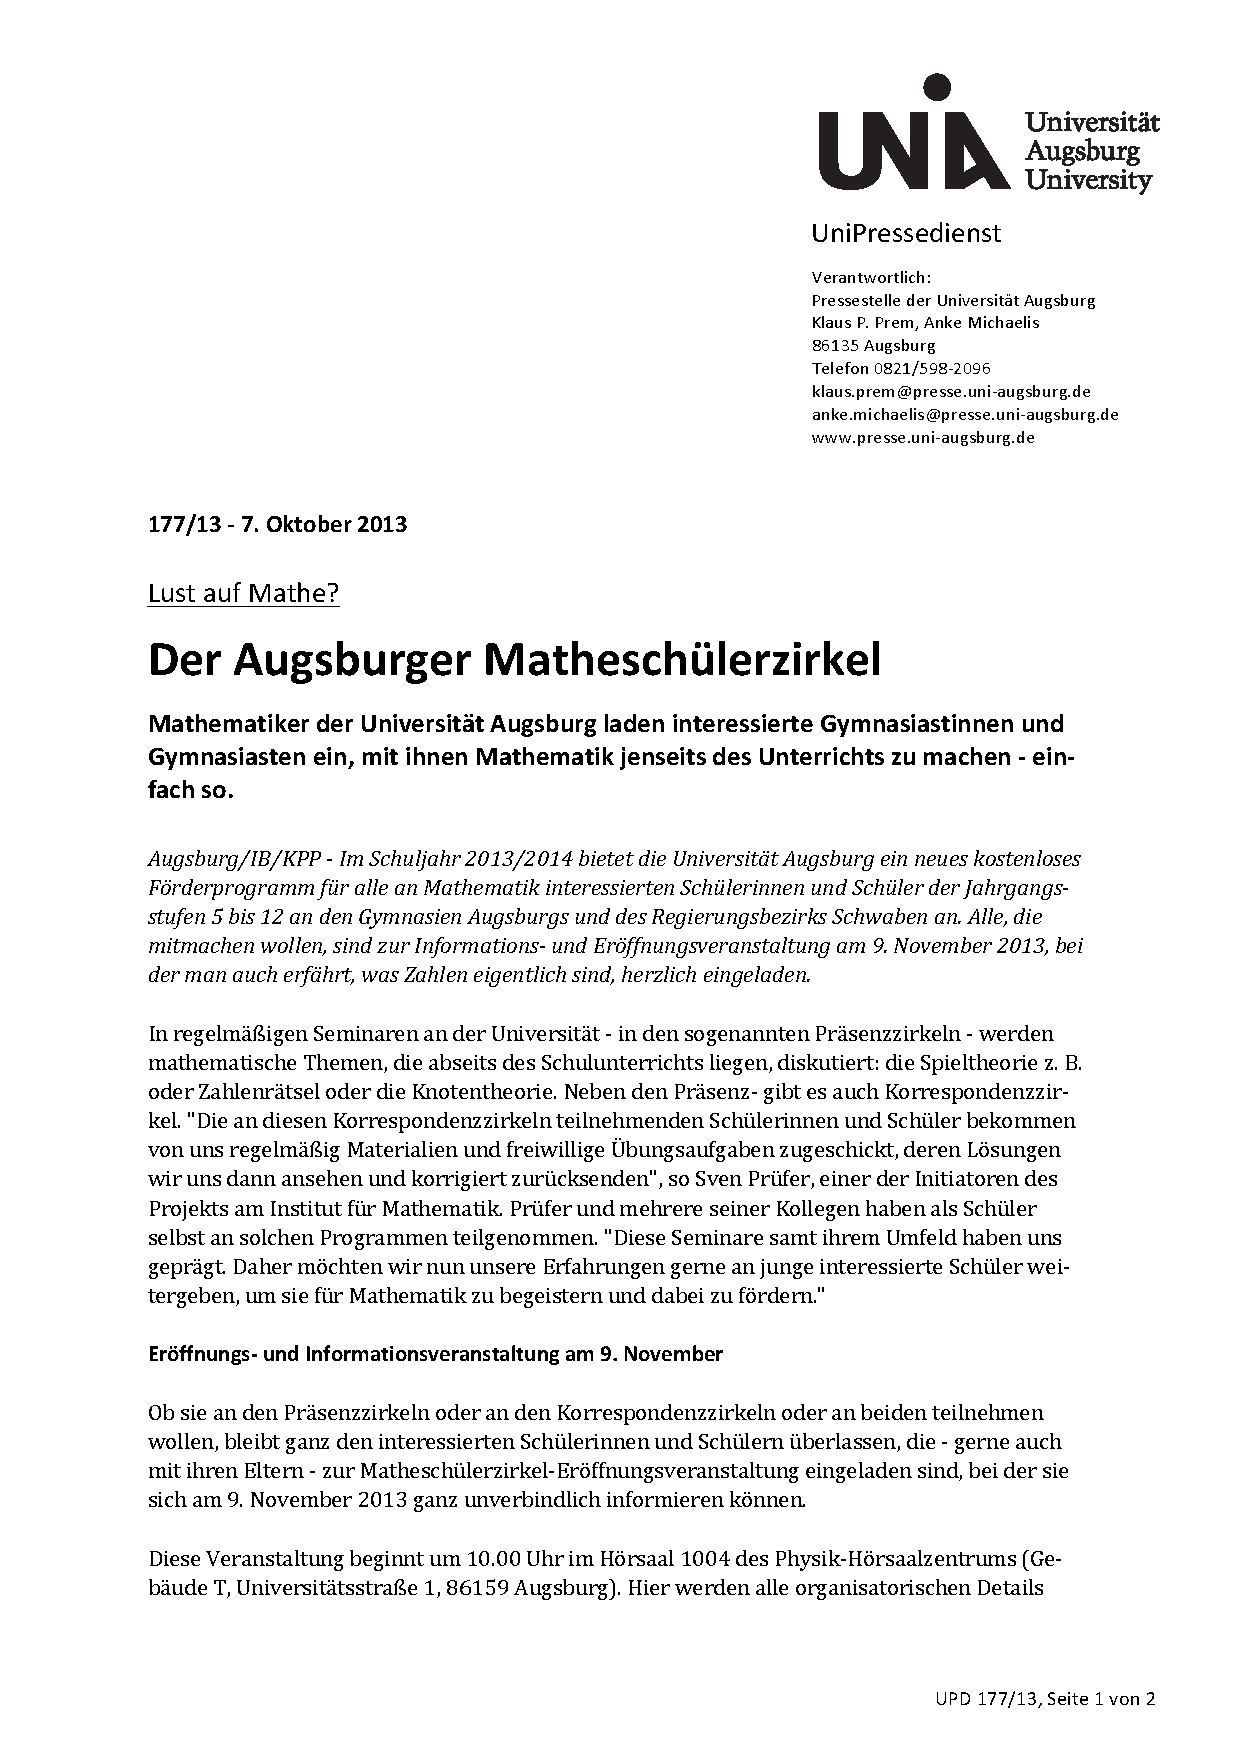
\includepdf[pages=1-2]{pressemitteilung-auftaktveranstaltung}

\pagestyle{empty}
\hspace{-3.5cm}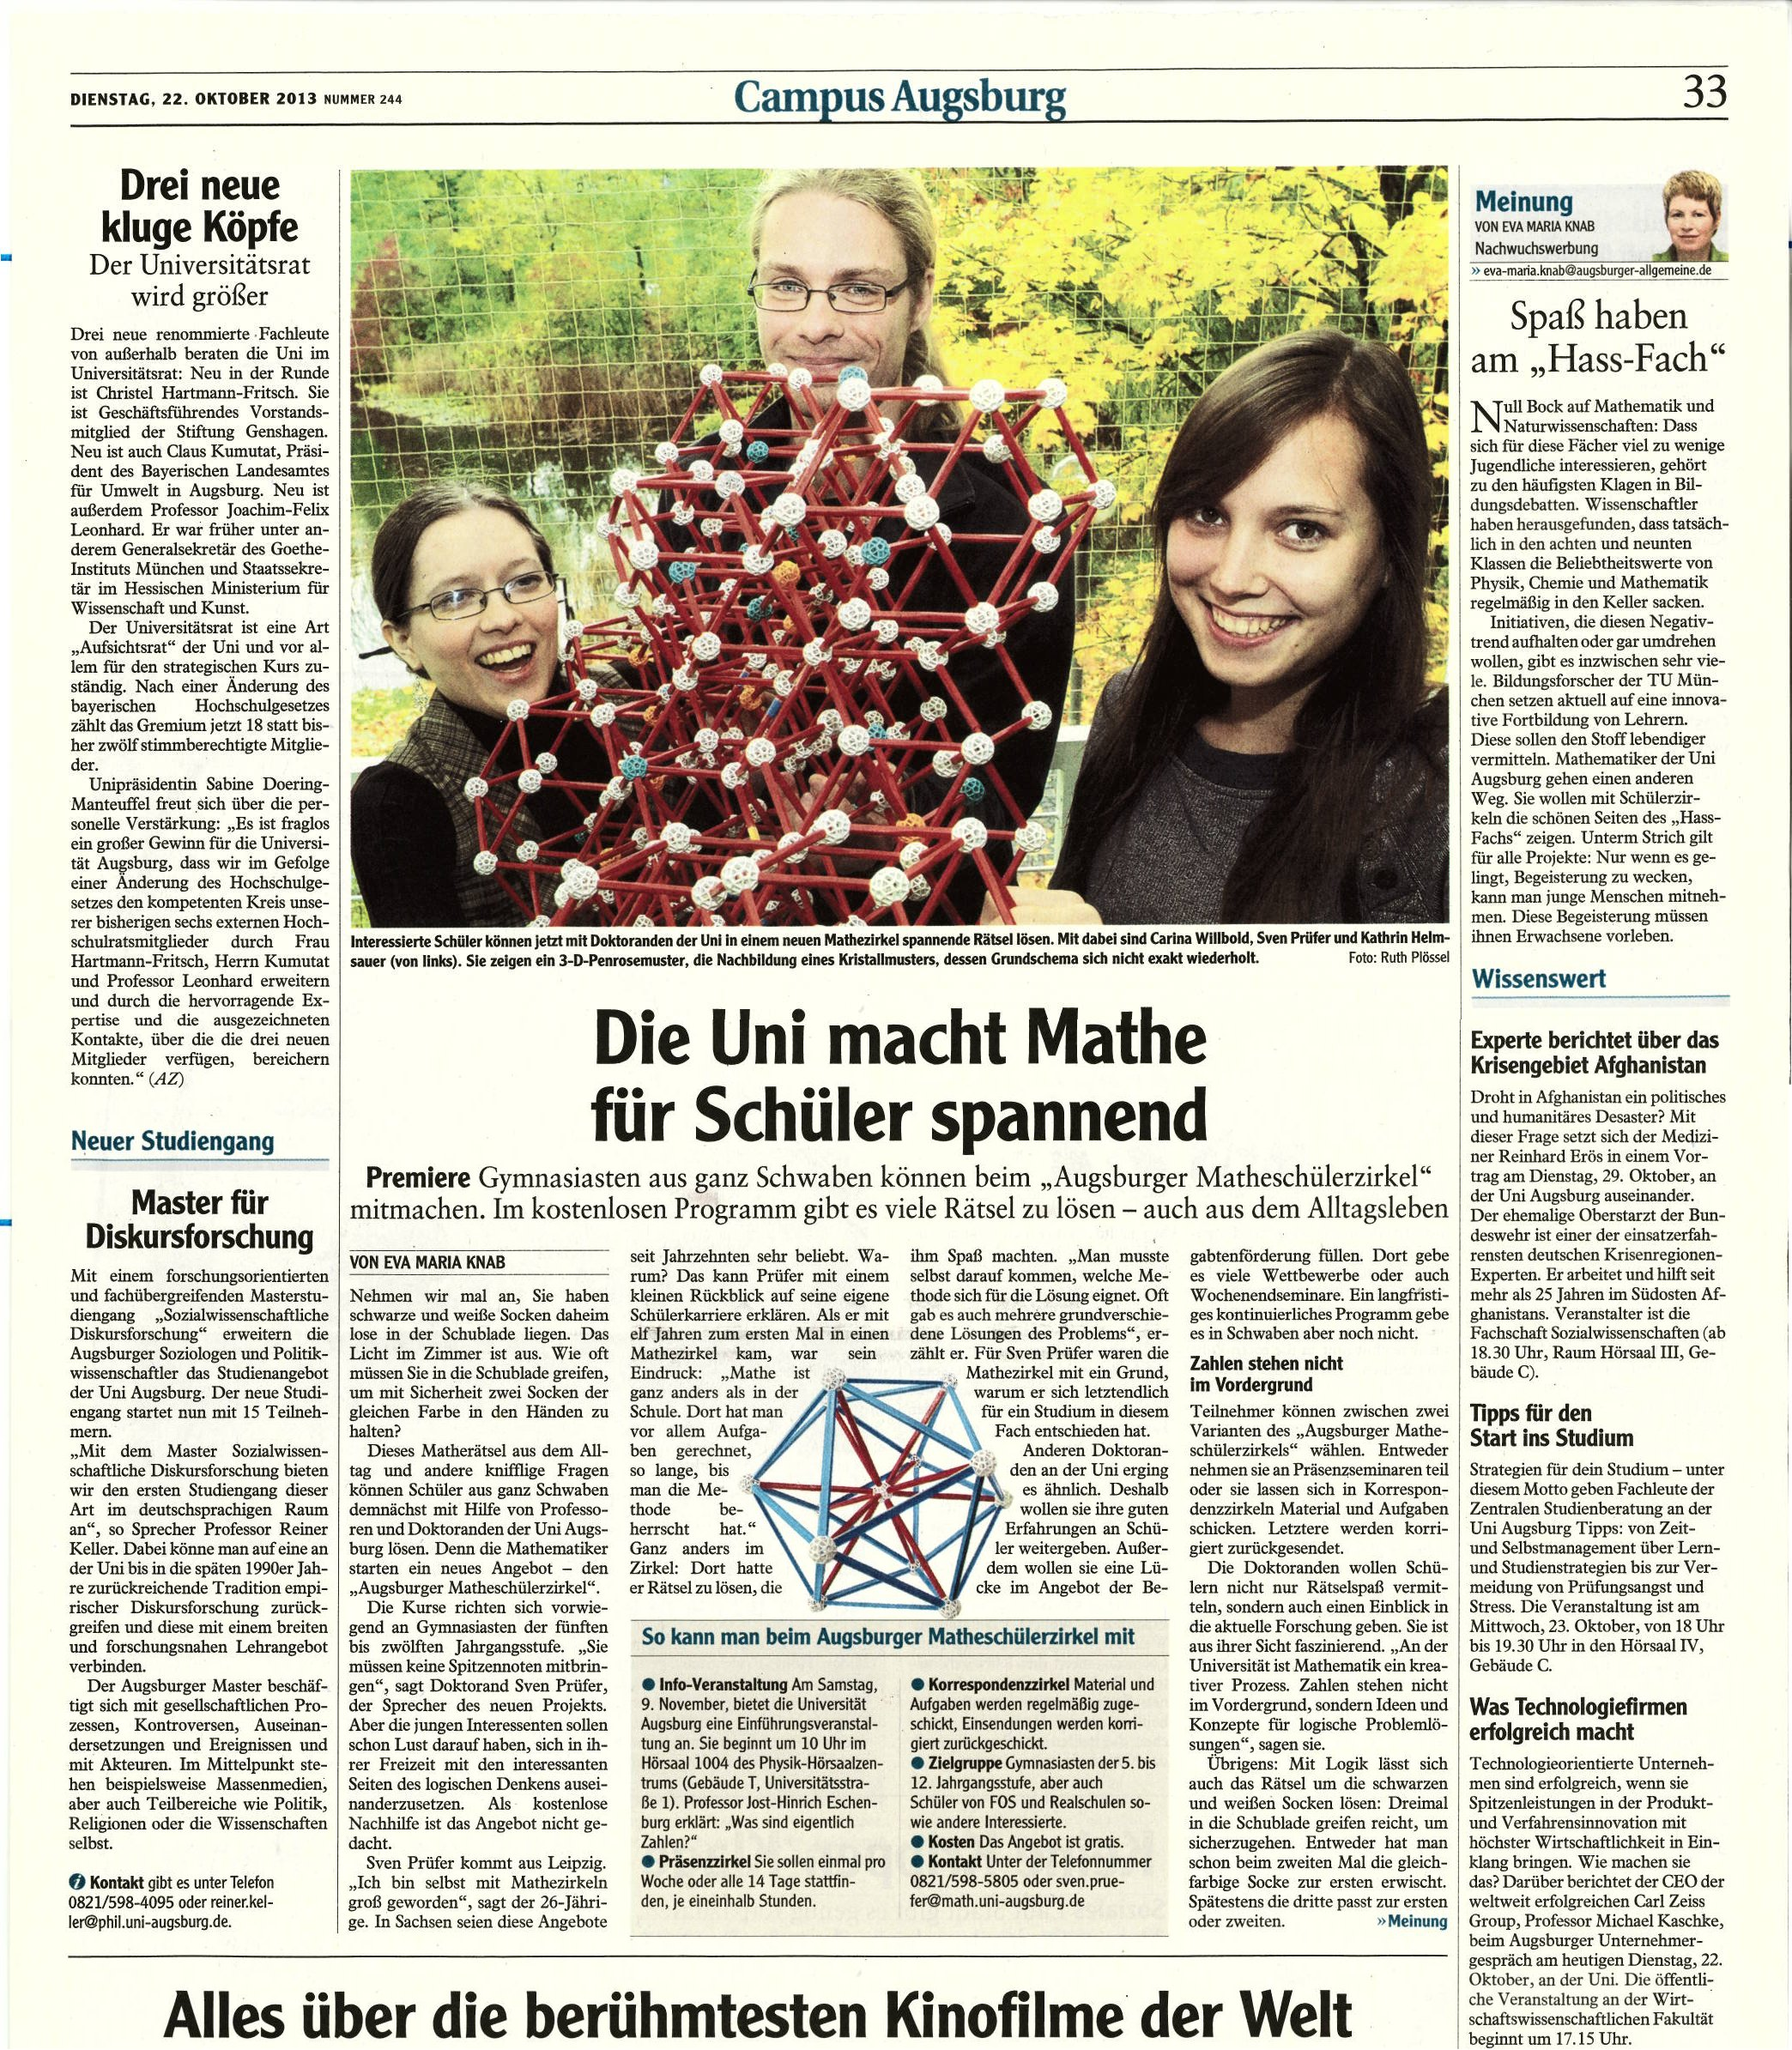
\includegraphics[scale=0.62]{Augsburger-Allgemeine-2013-10-22.jpeg}

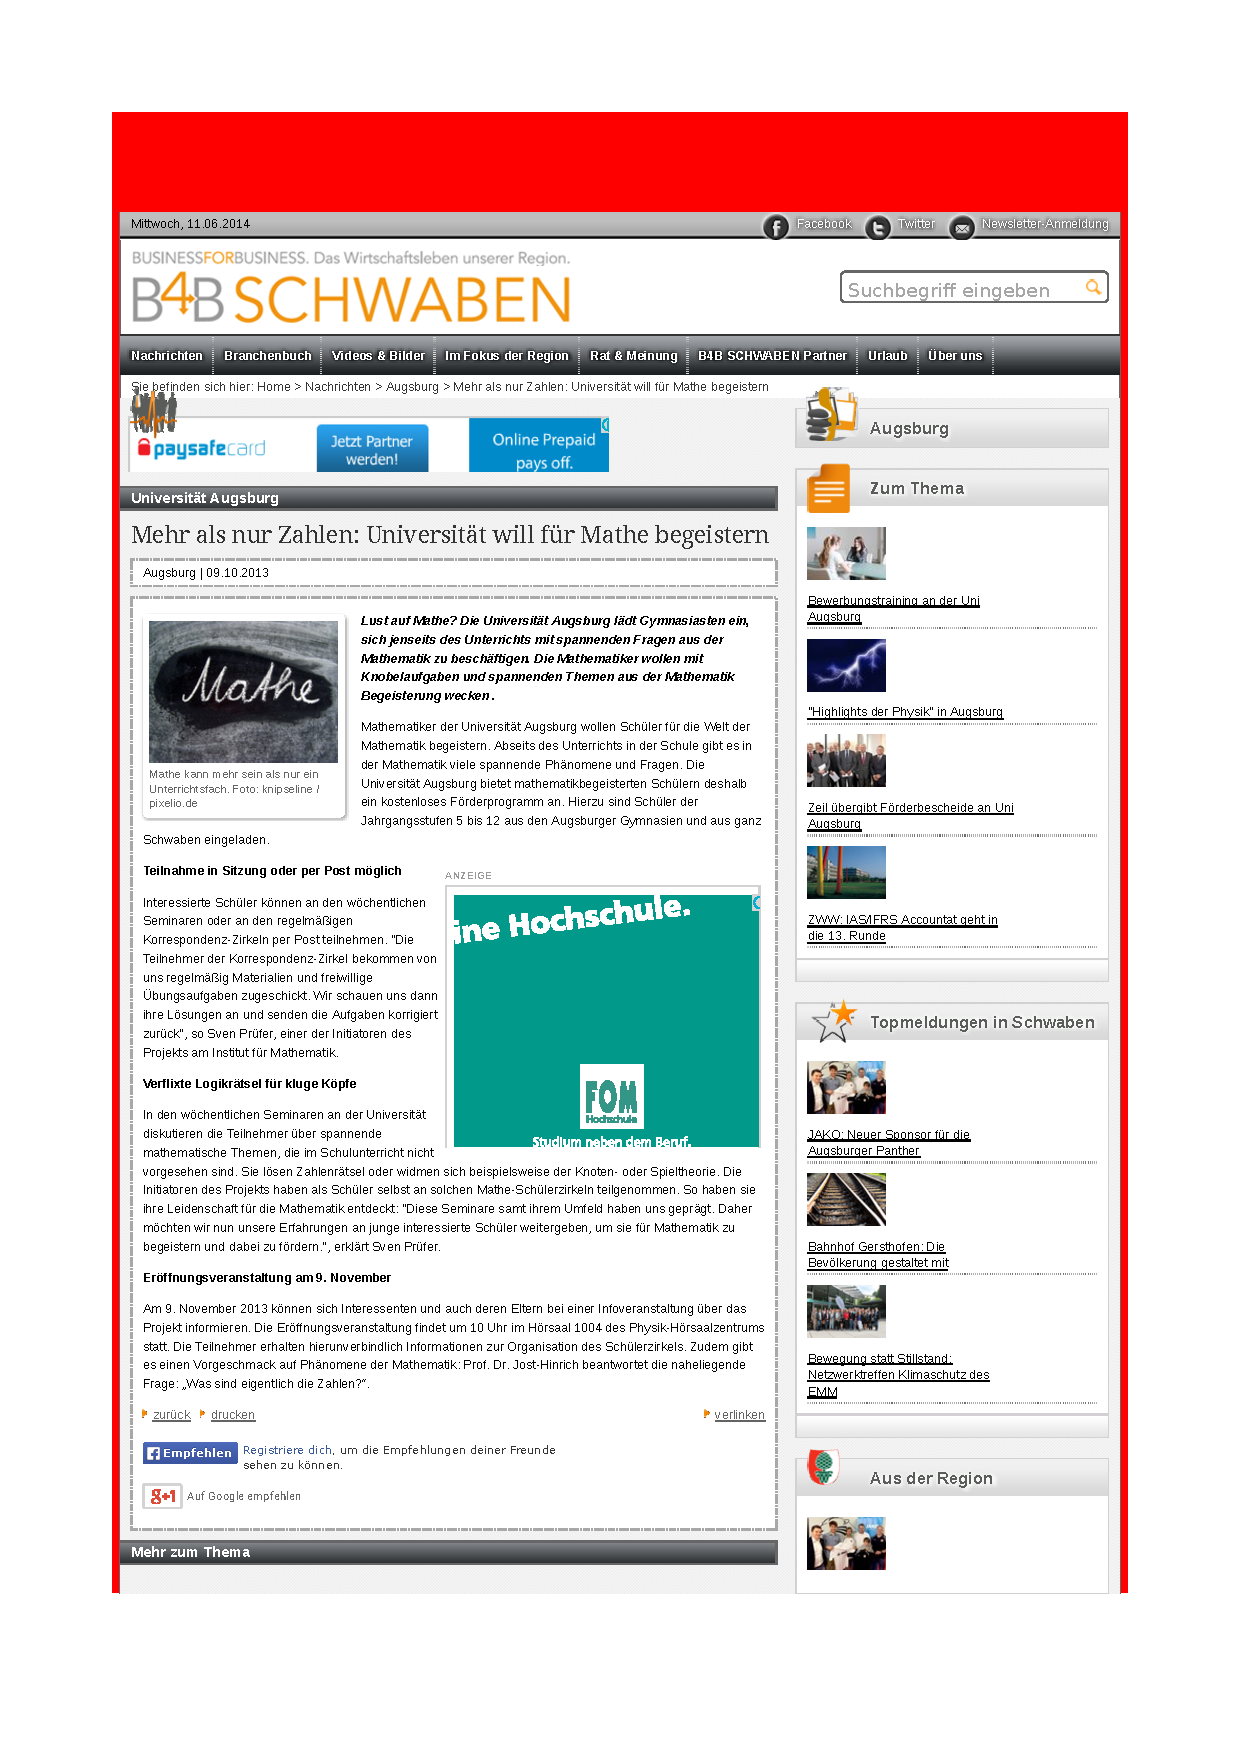
\includepdf{b4bschwaben-2013-10-09}

\end{document}
